\documentclass[amsmath,longbibliography,secnumarabic,floatfix,amssymb,nofootinbib,nobibnotes,letterpaper,11pt,notitlepage,tightenlines]{revtex4-1}

\usepackage[svgnames]{xcolor}
\usepackage{latexsym, amsmath, amscd, amsthm}
\usepackage{mathrsfs}
\usepackage{tikz}
\usepackage{pgfplots}
\usepackage{graphicx}
\usepackage{brunnian}
\usepackage{mathtools}
\usepackage{hyperref}
\usepackage{algorithmicx}
\usepackage{algpseudocode}
\usepackage{enumerate}

\setlength{\parskip}{.1cm}

\usetikzlibrary{decorations.markings,backgrounds,hobby}

\newcommand{\Z}{\mathbb{Z}} \newcommand{\N}{\mathbb{N}}

\newcommand{\UnkDia}{\mathcal{U}}
\newcommand{\TrefSum}{\mathcal{T}}
\newcommand{\KnotDia}{\mathcal{K}}
\newcommand{\FlatKnotDia}{\mathscr{K}}
\newcommand{\KnotShad}{\FlatKnotDia}
\newcommand{\LinkDia}{\mathcal{L}}
\newcommand{\LinkShad}{\mathscr{L}}
\newcommand{\ArbMaps}{\mathscr{M}}
\newcommand{\PrimeShad}{\mathscr{P}}
\newcommand{\ArbClass}{\mathscr{C}}
\newcommand{\ArbObj}{C}
\newcommand{\ArbSubClass}{\mathscr{D}}
\newcommand{\arbsubclass}{d}
\newcommand{\arbclass}{c}
\newcommand{\PatCount}{E}
\newcommand{\Prb}{\mathbb{P}}
\newcommand{\Shad}[1]{\tilde{#1}}
\newcommand{\FourTang}{\&}

\newcommand{\Expand}{T}
\DeclareMathOperator{\Aut}{aut}
\DeclareMathOperator{\im}{im}

\newtheorem{theorem}{Theorem}
\newtheorem{proposition}[theorem]{Proposition}
\newtheorem{lemma}[theorem]{Lemma}
\newtheorem*{lemma*}{Lemma}
\newtheorem{corollary}[theorem]{Corollary}
\newtheorem{definition}{Definition} \tikzset{->-/.style={decoration={ markings, mark=at position #1
      with {\arrow{>}}},postaction={decorate}}}

\begin{document}
%%% HEAD MATTER
\title[]{On the asymptotics of uniformly random knot diagrams} \author{Harrison Chapman}
\email{hchapman@math.uga.edu} \affiliation{Department of Mathematics\\University of Georgia, Athens
  GA}
% \noaffiliation{}
\date{\today}
%%%

\maketitle
\section{Introduction}
\label{sec:intro}

There is a dearth of models for drawing random knots; self avoiding lattice walks [cite], random
space polygons [cite], random braid words [cite], \emph{Petaluma} [cite], et.\ al. In this paper we
will discuss the \emph{random diagram model} under which \emph{knot diagrams} are drawn uniformly
from the set of all diagrams with a given number of crossings. Alternating knot and link diagrams
have been studied [cite] but little is published about the knottiness of arbitrary random diagrams
of large size.

In this paper we begin by considering a slightly different object, \emph{rooted diagrams}, which
break symmetries (as opposed to in \cite{CCMknotdiagrams2015}). We are then able to prove that in
the limit, knot diagrams behave similarly to rooted diagrams, so that these results carry over.

\section{Definitions}
\label{sec:defns}

\subsection{Preliminaries}
\label{sec:prelimdefs}

A \emph{knot} is an isotopy class of embeddings of the circle into $S^3$. A \emph{link} is an
isotopy class of embeddings of one or more circles into $S^3$. Both of the prior are considered up
to \emph{ambient isotopy} of the embedded circles. The study of links and knots is well known to be
equivalent to the study of \emph{link diagrams} and \emph{knot diagrams} (more formally defined
below) up to the so-called \emph{Reidemeister moves}. We wish to examine the underlying \emph{planar
  map} structure of knot and link diagrams;

\begin{definition}
  A \emph{planar map with $n$ vertices} $P$ is a graph $\tilde P$ embedded in the sphere. The planar
  map $P$ is \emph{4-regular} or \emph{quartic} if every vertex in the underlying graph $\tilde P$
  has degree 4. A \emph{rooted planar map} is a planar map together with a single edge marked with a
  direction.
\end{definition}

\begin{figure}[h!]
  \centering
  \begin{tikzpicture}[every path/.style={string, very thick}, every node/.style={transform shape,
      knot crossing, circle, fill=black, inner sep=2pt}]
    \begin{scope}
      \node (A) at (-1,0){};
      \node (B) at (0,1) {};
      \node (C) at (1,0) {};

      \node (D) at (-1,-2) {};
      \node (E) at (1,-2) {};

      \node (X) at (-2,-2) {};
      \node (Y) at (0, -1) {};
      \node (Z) at (-2,-1) {};

      \draw (A) -- (B) -- (C) -- (E) -- (D) -- (A);
      \draw (X) -- (D);
      \draw (A) -- (C);

      \draw (D) edge[out=90,in=180] (Y);
      \draw (D) edge[out=0,in=270] (Y);
      \draw (Y) edge[out=90,in=0,looseness=20] (Y);

      \draw (A) -- (Z);
      \draw (Z) edge[out=180+45,in=90+45,looseness=20] (Z);
      \draw (A) edge[out=90,in=180,looseness=20] (A);
    \end{scope}
    \begin{scope}[xshift=2in]
      % \draw[help lines,step=8pt] (-2,-2.6) grid (2.7,1);
      \useasboundingbox (-2,-2.6) rectangle (2.7,1);
      \node (A) at (-.8,0){};
      \node (B) at (0,-1) {};
      \node (C) at (.8,0) {};
      \node (D) at (0,-2) {};

      \node (Z) at (1.75,-1) {};

      \draw (A) -- (C);
      \draw (A) edge[out=75,in=105,looseness=1.3] (C);
      \draw (A) -- (B);
      \draw (C) -- (B);
      \draw (B) edge[out=180+45,in=90+45] (D);
      \draw (B) edge[out=270+45,in=45] (D);
      \draw (D) edge[out=180+45,in=180,looseness=2] (A);
      \draw (D) edge[out=270+45,in=-90,looseness=1.3] (Z);
      \draw (Z) edge[out=90,in=0,looseness=1.3] (C);
      \draw (Z) edge[out=-45,in=45,looseness=20] (Z);
    \end{scope}
  \end{tikzpicture}
  \caption{Two planar maps. The map on the right is in the class of knot shadows.}
  \label{fig:egplanarmaps}
\end{figure}

\begin{figure}[h!]
  \centering
  % \includegraphics[width=2in]{dual_to_fig8twist}
  \begin{tikzpicture}[every path/.style={string, thick, gray}, every node/.style={transform shape,
      knot crossing, circle, fill=gray, inner sep=2pt}]
    \begin{scope}
      % \draw[help lines,step=.2] (-2,-2.6) grid (3,1.2);
      \useasboundingbox (-2,-2.6) rectangle (2.7,1.2);
      \node (A) at (-.8,0){};
      \node (B) at (0,-1) {};
      \node (C) at (.8,0) {};
      \node (D) at (0,-2) {};

      \node (Z) at (1.75,-1) {};

      \draw (A) -- (C);
      \draw (A) edge[out=75,in=105,looseness=1.3] (C);
      \draw (A) -- (B);
      \draw (C) -- (B);
      \draw (B) edge[out=180+45,in=90+45] (D);
      \draw (B) edge[out=270+45,in=45] (D);
      \draw (D) edge[out=180+45,in=180,looseness=2] (A);
      \draw (D) edge[out=270+45,in=-90,looseness=1.3] (Z);
      \draw (Z) edge[out=90,in=0,looseness=1.3] (C);
      \draw (Z) edge[out=-45,in=45,looseness=20] (Z);
    \end{scope}
    \begin{scope}[every path/.style={string, very thick, black}, every
      node/.style={transform shape, knot crossing, circle, fill=black,
        inner sep=2pt}]
      \useasboundingbox (-2,-2.6) rectangle (2.7,1.2);
      \node (a) at (0,.4) {};
      \node (b) at (0,-.4) {};
      \node (c) at (-.8,-1) {};
      \node (d) at (.8,-1) {};
      \node (e) at (0,-1.5) {};
      \node (f) at (2.2,-1) {};
      \node (o) at (1.7, .4) {};

      \draw (a) -- (b) -- (c) -- (e) -- (d) -- (b);
      \draw (a) -- (o) -- (f);
      \draw (d) -- (o);
      \draw (d) edge[out=-80,in=0,looseness=3.8] (o);
      \draw (c) edge[out=150,in=120,looseness=1.5] (o);
    \end{scope}
  \end{tikzpicture}
  \caption{Planar quadrangulation which is dual to a knot shadow.}
  \label{fig:dualquadeg}
\end{figure}
Planar maps (indeed, maps on any surface) have a well defined notion of the \emph{dual map}; a map
$M = (V, E, F)$ has dual $M^* = (F, E^*, V)$, where there is an edge $(f_1, f_2) \in E^*$ if $f_1$
is adjacent to $f_2$ in $M$. The dual graph of a 4-regular planar map is a \emph{planar
  quadrangulation}.

\subsection{Diagrams and shadows}
\label{sec:shadowdefs}

By breaking symmetries with a root, we may study certain classes of planar maps by way of the
celebrated bijection with \emph{blossom trees}\cite{bouttier2003geodist}. We carry this idea to link
and knot diagrams:

\begin{figure}[h!]
  \centering
  % \includegraphics[height=1.4in]{planar_maps_rooted_ex}
  \begin{tikzpicture}[every path/.style={string, very thick}, every node/.style={transform shape,
      circle, fill=black, inner sep=2pt}]
    \begin{scope}[decoration={markings, mark=at position 0.5 with
        {\arrow{>}}}] \node (A) at (-1,0){}; \node (B) at (0,1) {}; \node (C)
      at (1,0) {};

      \node (D) at (-1,-2) {}; \node (E) at (1,-2) {};

      \node (X) at (-2,-2) {}; \node (Y) at (0, -1) {}; \node (Z) at
      (-2,-1) {};

      \draw (A) -- (B) -- (C) -- (E) -- (D) -- (A); \draw (X) -- (D);
      \draw (A) -- (C);

      \draw (D) edge[out=90,in=180] (Y); \draw (D) edge[out=0,in=270]
      (Y); \draw (Y) edge[out=90,in=0,looseness=20] (Y);

      \draw (A) -- (Z); \draw (Z)
      edge[postaction={decorate},out=180+45,in=90+45,looseness=20] (Z);
      \draw (A) edge[out=90,in=180,looseness=20] (A);
    \end{scope}
    \begin{scope}[xshift=2in,decoration={markings, mark=at position
        0.5 with {\arrow{<}}}] %\draw[help lines,step=8pt] (-2,-2.6) grid
      (2.7,1); \useasboundingbox (-2,-2.6) rectangle (2.7,1); \node (A) at
      (-.8,0){}; \node (B) at (0,-1) {}; \node (C) at (.8,0) {}; \node (D)
      at (0,-2) {};

      \node (Z) at (1.75,-1) {};

      \draw (A) -- (C); \draw (A) edge[out=75,in=105,looseness=1.3]
      (C); \draw (A) -- (B); \draw (C) -- (B); \draw (B)
      edge[out=180+45,in=90+45] (D); \draw (B) edge[out=270+45,in=45] (D);
      \draw (D) edge[out=180+45,in=180,looseness=2] (A); \draw (D)
      edge[out=270+45,in=-90,looseness=1.3] (Z); \draw (Z)
      edge[postaction={decorate},out=90,in=0,looseness=1.3] (C); \draw (Z)
      edge[out=-45,in=45,looseness=20] (Z);
    \end{scope}
  \end{tikzpicture}
  \caption{Two rooted planar maps. The map on the right is in the class of rooted knot shadows.}
  \label{fig:egrootedplanarmaps}
\end{figure}

\begin{definition} A \emph{(rooted) link diagram with $n$ crossings} is a 4-regular (rooted) planar
  map of $n$ vertices together with a choice of over-under strand information at each vertex. The
  class of rooted link diagrams with $n$ crossings is denoted $\LinkDia_n$.

  The class of maps which represent rooted \emph{link shadows} in $n$ crossings, i.e.\ maps which
  can be found as the underlying map structure of a rooted link diagram are denoted $\LinkShad_n$.
\end{definition} It is well understood that the class of rooted link shadows in $n$-vertices is
identical to the class of 4-regular planar maps in $n$ vertices is identical to $\LinkShad_n$;
furthermore, the class of rooted planar quadrangulations is dual to $\LinkShad_n$.
\begin{definition} A \emph{(rooted) knot diagram} is a (rooted) link diagram which consists of only
  one knot component. The class of rooted knot diagrams with $n$ crossings is denoted by
  $\KnotDia_n$.

  The class of maps which represent rooted \emph{knot shadows} in $n$ crossings are denoted
  $\KnotShad_n$.
\end{definition} Knot shadows $\KnotShad_n$ represent a curious, small subclass of $\LinkShad_n$.

Rooted (knot or link) diagrams are equivalently viewed as \emph{two-leg diagrams} or
\emph{2-tangles} as illustrated below.
\begin{figure}[h!]  \centering
  \begin{tikzpicture}[every path/.style={string, very thick}, every node/.style={transform shape,
      knot crossing, inner sep=1.5pt}]
    \begin{scope}[xshift=-1.5in] \node (tl) at (-.7,0) {}; \node (tr)
      at (.7,0) {}; \node (tc) at (0,1) {}; \draw (tl) .. controls (tl.4
      north east) and (tc.4 south west) ..  (tc.center); \draw (tc.center)
      .. controls (tc.8 north east) and (tr.8 north east) .. (tr); \draw
      (tr) .. controls (tr.4 south west) and (tl.4 south east)
      .. (tl.center); \draw (tl.center) .. controls (tl.8 north west) and
      (tc.8 north west) .. (tc); \draw (tc) .. controls (tc.4 south east)
      and (tr.4 north west) .. (tr.center); \draw[->-=.5] (tr.center)
      .. controls (tr.16 south east) and (tl.16 south west) .. (tl);
    \end{scope}

    \begin{scope}[xshift=1.5in] \node (tl) at (-.7,0) {}; \node (tr)
      at (.7,0) {}; \node (tc) at (0,1) {}; \node (el) at (-1.7,0) {}; \node
      (er) at (1.7,0) {}; \draw[>-] (el.center) .. controls (el.4 east) and
      (tl.4 south west) .. (tl); \draw (tl) .. controls (tl.4 north east)
      and (tc.4 south west) ..  (tc.center); \draw (tc.center) .. controls
      (tc.8 north east) and (tr.8 north east) .. (tr); \draw (tr)
      .. controls (tr.4 south west) and (tl.4 south east) .. (tl.center);
      \draw (tl.center) .. controls (tl.8 north west) and (tc.8 north west)
      .. (tc); \draw (tc) .. controls (tc.4 south east) and (tr.4 north
      west) .. (tr.center); \draw[->] (tr.center) .. controls (tr.4 south
      east) and (er.4 west) .. (er.center);
    \end{scope} \draw[<->] (-1.6,.3) -- (1,.3) node[text
    width=3cm,text centered,midway]{cut/splice root edge};
  \end{tikzpicture}
  \caption{Rooted diagrams of the trefoil and its mirror image}
  \label{fig:treflegs2}
\end{figure}

Additionally, rooted diagrams can be viewed as \emph{four-leg diagrams}, or \emph{$4$-tangles} by
deleting the root crossing. This identification is not injective for diagrams as it forgets the sign
of the removed crossing.

A (rooted) shadow is \emph{prime} if it cannot be disconnected by removing two edges (i.e.\ it is at
least 3-connected); otherwise it is \emph{composite}. A rooted shadow is \emph{two-leg-prime} if it
cannot be disconnected by removing two edges, one being the root edge. Diagrams are (two-leg-)prime
if their underlying shadow structure is.

\begin{figure}[h!]  \centering
  \includegraphics[height=1.5in]{2leg_vs_reg_prime}
  \caption{A composite shadow which is two-leg-prime (left). A shadow
    which is not two-leg-prime (right). }
  \label{fig:prime2legprime}
\end{figure}

There is a bijection between blossom trees and rooted link shadows.

\begin{proposition}
  There is a consistent way to order the components of a rooted link
  shadow. There is a consistent way to index the vertices of a rooted
  link shadow. There is a consistent way to index and orient the edges
  of a rooted link shadow so that the directed edges meet head-to-tail
  across the vertices of the shadow.
  \label{prop:canonicalori}
\end{proposition}

\begin{proof}
  Let $L$ be a rooted link shadow. Begin by labelling the edges of $L$
  with the link component in which they lie. Index the root vertex and
  the root edge by 1.
\end{proof}

\begin{corollary}
  There is a consistent way to order and orient the components of a
  rooted link diagram. There is a consistent way to index the
  crossings of a rooted link diagram. There is a consistent way to
  index the edges of a rooted link diagram. These are the same as
  those for the underlying shadow.
\end{corollary}

\begin{proof}
  These are all induced on the diagram from its shadow.
\end{proof}

\begin{corollary}
  Rooted link diagrams are in bijection with rooted link shadows
  labelled with $\{+, -\}$.
\end{corollary}

\begin{proof}
  Given a rooted link diagram, there is a consistent orientation of
  its components. There is hence a labelling of the underlying rooted
  shadow with $\{+, -\}$ (they are the standard crossing signs). This
  process is reversible since the consistent component orientation for
  the diagram is identical to that of the shadow.
\end{proof}

\section{Asymptotic structure theorems for diagrams}
\label{sec:structure}

It is believed and numerically evident \cite{PZJasympconj2004} that the number of link diagrams in a
random link diagram grows exponentially, hence a random link diagram is almost certainly not a knot
diagram.

\subsection{A pattern theorem for classes of link diagrams}
\label{sec:patternthm}

\newcommand{\MapClass}{\mathscr{M}}

\subsubsection{A pattern theorem}
\label{sec:weakpatternthm}

Theorem 2 in \cite{Bender1992104} provides a pattern theorem for knot and link shadows, provided a
strategy of attaching a desired pattern. However, care is required in the case of knot or link
\emph{diagrams}, in which each vertex takes a value in the set $\{+, -\}$. In fact, we turn our
attention to the dual case in which \emph{faces} are labelled with an arbitrary set.

\begin{definition}
  Given a triple of label sets $S = (S_V, S_E, S_F)$, an
  \emph{$S$-map} is a map $M = (V,E,F)$ together with a triple of maps
  $(s_V, s_E, s_F)$, $s_*: * \to S_*$ which label each vertex, edge,
  and face of $M$ with an element of $S$.
\end{definition}

\begin{theorem}Let $S$ be a set and $\MapClass[S]$ be some class of
  $S$-maps on a surface of type $g$ and let $P$ be a planar $S$-map
  with boundary that can be found as a submap of maps in
  $\MapClass[S]$. Let $M(x)$ be the generating function by number of
  edges for $\MapClass$. Let $H(x)$ be the generating function by
  number of edges for those maps $M$ in $\MapClass[S]$ that contain
  less than $ce(M)$ pairwise disjoint copies of $P$. Suppose that we
  can embed $P$ in a possibly larger rooted planar labeled map with
  boundary $Q$ and attach copies of $Q$ to each map $K$
  counted by $H(x)$ in such a way that
  \begin{enumerate}
  \item for some fixed positive integer $k$, at least $\lfloor e(K)/k \rfloor$ possible
    non-conflicting places of attachment exist,
  \item only $S$-maps in $\MapClass[S]$ are produced,
  \item for any map produced as such we can identify the copies of $Q$ that have been added and they
    are all pairwise disjoint, and
  \item given the copies that have been added, the original map and associated places of attachment
    are uniquely determined.
  \end{enumerate} If $1 > c > 0$ is sufficiently small, then $r(M) < r(H)$. The maps may be rooted or
  not.
  \label{thr:weakpattern}
\end{theorem}

The method of attachment is vague, but flexible. We will provide some examples which we use in our
results for knot diagrams. The proof extends the proof of the original theorem for maps, and makes
use of a lemma:


\begin{lemma*}[\cite{Bender1992104}, lemma 3]
 If
 \begin{enumerate}
 \item $F(z) \ne 0$ is a polynomial with non-negative coefficients and $F(0) = 0$,
 \item $H(w)$ has a power series expansion with non-negative coefficients and $0 < r(H) < \infty$,
 \item for some positive integer $k$ the linear operator $\mathscr{L}$ is given by $\mathscr{L}(w^n)
   = z^n(F(z)/z)^{\lfloor n/k \rfloor}$, and
 \item $G(z) = \mathscr{L}(H(w))$,
 \end{enumerate}
 then $r(H)^k = r(G)^{k-1}F(r(G))$.
\end{lemma*}

The proof of the theorem then remains almost unchanged from the original theorem, although care will
be necessary in defining attachment.

\begin{proof}[Proof of theorem \ref{thr:weakpattern}.]
  Let $G(z)$ be the generating function which counts $S$-maps $\mathscr{G}[S]$ which are the
  result of attaching some number between $0$ and $\lfloor n/k \rfloor$ copies of $Q$ to $S$-face
  maps $\mathscr{H}[S]$ counted by $H(x)$. The method of
  attachment leads to the relation $G(z) = \mathscr{L}(H(w))$, where $F(z) = z + z^q$ and $q$ is the
  number of edges added when a copy of $Q$ is attached, as
  \[ G(z) = \sum_{X \in \mathscr{G}[S]}{z^{e(X)}} = \sum_{Y \in \mathscr{H}[S]}{z^{e(Y)}\left( 1 +
      z^{q-1} \right)^{\lfloor n/k \rfloor}} = \mathscr{L}(H(w)).\]
  Let $g_n$ be the coefficients of $G(z)$.

  Suppose $M \in \MapClass[S]$ contains $m$ copies of $Q$. By property (3) of our attachment, $m \le
  n$. If $M$ had been produced from some $S$-map $K$ in $\mathscr{H}[S]$ by our attachment
  process, we can find all possible $K$ by removing at least $m - cn$ copies of $Q$ from $M$. It is
  possible to bound from above the number of ways to do this by
  \[ \sum_{j \ge m-cn}{\binom m j} = \sum_{k < cn}{\binom m k} < \sum_{k < cn}{\binom n k} \le
  {n\binom n{cn}} \le \frac{n(ne)^{cn}}{{cn}^{cn}} = n\left(\frac ec\right)^{cn} =: t_n.\] If $M(x)
  = \sum{m_nx^n}$, then $m_n \ge g_n$ and $t_n > 1$ for sufficiently large $n$, so $m_n \ge
  g_n/t_n$. Hence,
  \[1/r(M) \ge \limsup_{n \to \infty}{(g_n/t_n)^{1/n}} = \lim_{n \to \infty}{(t_n)^{-1/n}}\limsup_{n
    \to \infty}{(g_n)^{1/n}} \ge (c/e)^c/r(G).\]
  By the prior lemma, $r(H)^k = r(G)^k(1 + r(G)^{q-1})$ so that
  \[ r(H)/r(M)\ \ge (1 + r(G)^{q-1})^{1/k} (c/e)^c. \]
  As $\lim_{c \to 0^+}{(c/e)^c} = 1$ and $r(G)^k(1 + r(G)^{q-1}) = r(H)^k \ge 1/12^k$, it follows
  that $r(H)/r(M) > 1$ for sufficiently small $c$, completing the proof of the theorem.
\end{proof}

The conclusion is about radii of convergence of two power series, and may appear an esoteric
result. However, application of the Cauchy-Hadamard theorem, together with one additional
hypothesis, gives a more familiar tune:

\begin{corollary}[\cite{Bender1992104}]
  Suppose all of the hypotheses of theorem \ref{thr:weakpattern} and additionally that $\MapClass[S]$
  grows smoothly, i.e.\ that $\lim_{n\to\infty}{m_n^{1/n}}$ exists. Then there exists constants $c >
  0$ and $d < 1$ and $N > 0$ so that for all $n \ge N$,
  \[ \frac{h_n}{m_n} < d^n. \]
  I.e., the pattern $P$ is \emph{ubiquitous}.
\end{corollary}

Because of Euler's formula, the number of vertices, edges, or faces in a link shadow or planar
quadrangulation is entirely determined by choosing any one cardinality. Hence, we can size shadows
by the number of vertices and still keep the above results.

The crux of applying this theorem to link diagrams then falls upon
determining an ``attachment'' operation which satisfies the
hypotheses, along with patterns valid for a given class of shadows.
We can generally define attachment operations for different kinds of
tangles in the dual. By abuse of notation, let $S = (\{0\}, \{0\}, S)$ be a set of
labels for the faces of the dual (for now, we are concerned about
diagrams, which only have labeled vertices).
\begin{enumerate}
\item \textbf{Connect sum.} Let $L$ and $Q'$ be rooted $S$-quadrangulations. Orient the
  remaining edges of $L$ canonically by proposition~\ref{prop:canonicalori}. Define the
  \emph{connect sum} of $Q'$ into $L$ at an edge $e \in L$, $L \#_e Q'$, by
  \begin{enumerate}
  \item Cut and split the edge $e$, creating a map $L'$ and leaving a distinguished, oriented bigon
    $f$. Denote the two edges formed by splitting $e$ by $e_1$, $e_2$, so that the loop $e_1(-e_2)$
    is a counterclockwise cycle around $f$. If $e$ was the root of $L$, make $e_1$ the new root of
    $L'$.
  \item Cut and split the root edge $\epsilon$ of $Q'$, creating a map $Q$ and leaving a
    distinguished, oriented bigon $g$. Denote the two edges formed by splitting $\epsilon$ by
    $\epsilon_1, \epsilon_2$, so that the loop $\epsilon_1(-\epsilon_2)$ is a counterclockwise cycle
    around $g$. Make $\epsilon_2$ the new root of $Q$.
  \item Glue the map $Q$ into the map $L'$'s distinguished face $f$ along the boundary of the
    distinguished bigon $g$ so that $e_1$ and $\epsilon_2$ are mapped to the same edge and so that
    the orientations of the boundaries align.
  \item Forget about all edge orientations except for the root edge of $L$.
  \end{enumerate} Notice that none of the original faces in $L$ and $Q'$ are changed; hence the
  result is a new rooted $S$-quadrangulation. Any given $S$-quadrangulation in $2n$ edges
  has precisely $2n$ different non-conflicting sites for connect summation (i.e. $k = 1$ for this
  attachment operation). This process is reversible, given a 2-cycle which bounds an instance of
  $Q'$ (collapse the disk to a single edge).
  \begin{figure}[h!]  \centering
    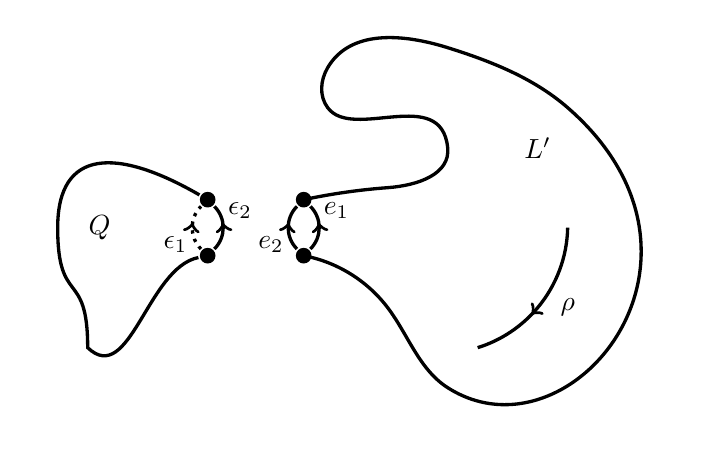
\begin{tikzpicture}
      % \node[anchor=south west, inner sep=0] (img) at (0,0)
      % {\includegraphics[height=2in]{connect_sum_topology}};x={(img.south east)},y={(img.north
      % west)},
      \begin{scope}[x={(3in,0in)},y={(0in,2in)},every
        node/.style={circle,fill=black,inner sep=2pt},every
        path/.style={black,very thick},decoration={markings, mark=at position
          0.6 with {\arrow{>}}}]
        % \draw[help lines,xstep=.1,ystep=.1] (0,0) grid (1.1,1);
        \useasboundingbox (0,0) rectangle (1.1,1);
        \node (L_A) at (.46,.43) {};
        \node (L_B) at (.46,.57) {};
        \draw[out=90+45,in=180+45,postaction={decorate}] (L_A) to node[fill=none,midway,below left]{$e_2$} (L_B);
        \draw[out=90-45,in=-45,postaction={decorate}] (L_A) to node[fill=none,midway,above
        right]{$e_1$} (L_B);
        \node[fill=none] (L_L') at (.85,.7) {$L'$};
        \draw[hobby,postaction={decorate}] plot coordinates {(.9,.5) (.85,.3) (.75,.2)};
        \node[fill=none] (root) at (.9,.3) {$\rho$};


        % \draw (L_B) .. controls (.7,.6) and (.7,.75) .. (.6,.8)
        % .. controls +(130:.2) and +(270:.1) ..
        % (.5,.9) -- (.9,.9) -- (.9,.2) -- (L_A);
        \draw[hobby] plot coordinates {(L_B) (.6,.6) (.7,.7) (.5,.8)
          (.5,.9) (.7,.95) (.9,.8) (.7,.1) (.6,.3) (L_A)};

        \node (Q_A) at (.3,.43) {};
        \node (Q_B) at (.3,.57) {};
        \draw[out=90-45,in=-45,postaction={decorate}] (Q_A) to node[fill=none,midway,above right]{$\epsilon_2$} (Q_B);
        \draw[dotted,out=90+45,in=180+45,postaction={decorate}] (Q_A) to
        node[fill=none,midway,below left]{$\epsilon_1$} (Q_B);
        \draw (Q_B) .. controls (.15,.7) and (.05,.7) .. (0.05,.5)
        .. controls (.05,.3) and (.1,.4) .. (.1,.2) .. controls
        (.17,.1) and (.2,.4) .. (Q_A);
        \node[fill=none] (Q_Q') at (.12,.5) {$Q$};

      \end{scope}
    \end{tikzpicture}
    \caption{The connect sum operation. $Q'$ and $L'$ are viewed as CW-complexes, and their
      boundaries are appropriately identified.}
    \label{fig:cs_topology}
  \end{figure}
  If $L^*$ and $(Q')^*$ each consist of only one link component, then
  $(L\#_eQ')^* =: L^*\#_e(Q')^*$ will as well. In fact, this
  attachment into the quadrangulation is precisely dual to the usual
  link connect sum from knot theory. If $Q$ is 2-leg prime, then no
  two copies of $Q$ can intersect (as in this case there are precisely
  two paths of length 1 in $Q$ between its two boundary vertices).

\item \textbf{4-tangle replacement.} Let $L$ be a rooted
  $S$-quadrangulation, and $Q$ a rooted $S$-quadrangulation with
  square boundary. Then given a face $f \in L$, we can define a
  \emph{4-tangle replacement} of $f$ with $Q$ by identifying the
  boundary of $Q$ with the boundary of $f$ in some manner. Precisely
  how to equate the boundaries will depend on the case at hand; what
  matters is that there be at least one valid way to glue $Q$ into any
  face $f$ and produce a new $S$-quadrangulation in the chosen
  class. Indeed, the result will always be a new
  $S$-quadrangulation. Any $S$-quadrangulation in $2n$ edges has $n$ faces, and hence at
  least $n$ non-conflicting attachment locations (i.e., $k = 2$).

  To make the process reversible for all $S$ (not just $S = \{0\}$),
  we must pick slightly different $Q$. Given a non-trivial $S$-map
  $P$, choose a planar rooted labeled map with boundary $Q$ which cannot
  intersect with a copy of itself so that $P$ is a unique copy of
  itself in $Q$, where all faces which are not in $P$ are labeled
  with a special label $*$. Attachment of $Q$ into the face $f$ of an
  $S$-quadrangulation $L$ then consists first of the actual attachment
  operation described above, and then relabeling all faces with label
  $*$ with the original label of $f$. The process is then reversed by
  \begin{enumerate}
  \item Given a 4-cycle bounding a (relabeled) copy $Q'$ of $Q$ in
    $L$, tentatively delete the copy and replace it with a bare face
    $f$.
  \item Identify the unique copy of $P$ inside of $Q$.
  \item If every face of $Q \setminus P$ does not have the same
    label $x$, then this would not in fact have been a place of attachment
    (hence reversal needn't be possible). If they do, then label the
    new face $f$ with the label $x$.
  \end{enumerate}

  Care must be taken in choice of $Q$ in which to embed arbitrary $P$
  here; an important fact to remember is that submap insertion of any
  $S$-quadrangulation with boundary $P$ will not introduce any shorter
  paths through $Q$, else there would be a $3$-cycle in $P$ (which is
  impossible as it is a quadrangulation).

  If one is dealing with 4-tangle replacement within a class of knot
  $S$-shadow duals, the following lemma is helpful;
  \begin{lemma}
    Given a link $S$-shadow $L$, a vertex $v$ in $L$, and an 4-leg
    $S$-curve $T$ with 2 link components, it is always possible to
    replace $v$ by $T$ in at least one way so that the result has the
    same number of components as $L$.
  \end{lemma}
  \begin{proof}
    TODO: This proof needs work

    The vertex $v$ in $L$ and the tangle $T$ are each either of
    crossing (abab) type or tangency (aabb) type. If they agree in
    type, replace $v$ by $T$ so that the strands agree. If they differ
    and $L \setminus v$ is of type abab, replace $T$ in with type
    abba. If they differ and $L \setminus v$ is of type aabb, replace
    $T$ with type abab. In all cases, the number of components is
    preserved.
  \end{proof}


  There are applications of this attachment in proving the weak
  pattern theorem for certain classes of maps:
  \begin{enumerate}[i.]
  \item Given arbitrary face labels $S$, a prime link dual $S$-shadow $L$
    and a prime 4-leg dual $S$-curve $P$,
    define $Q$ as in figure~\ref{fig:linktangrep}.
    \begin{figure}[h!]
      \centering
      % \includegraphics[width=2in]{dual_to_fig8twist}
      \begin{tikzpicture}[every path/.style={string, thick, gray}, every node/.style={transform shape,
          knot crossing, circle, fill=gray, inner sep=2pt}]
        \begin{scope}
          % \draw[red,step=.5] (-2,-2) grid (2,2);
          \useasboundingbox (-2,-2) rectangle (2,2);
          \node[fill=none,draw=gray,minimum size=20pt] (O) at (0,0) {};
          \node[fill=none] (LL) at (-2,0) {};
          \node (L) at (-1,0){};
          \node (R) at (1,0) {};
          \node[fill=none] (RR) at (2,0) {};
          \node[fill=none] (UU) at (0,2) {};
          \node (U) at (0,1) {};
          \node (D) at (0,-1) {};
          \node[fill=none] (DD) at (0,-2) {};

          \draw (LL) -- (L) -- (O) -- (R) -- (RR);
          \draw (UU) -- (U) -- (O) -- (D) -- (DD);
          \draw (L) edge[out=90,in=180] (U);
          \draw (U) edge[out=0,in=90] (R);
          \draw (R) edge[out=-90,in=0] (D);
          \draw (D) edge[out=180,in=-90] (L);
        \end{scope}
        \begin{scope}[every path/.style={string, very thick, black}, every
          node/.style={transform shape, knot crossing, circle, fill=black,
            inner sep=2pt}, decoration={markings, mark=at position 0.4 with
            {\arrow{<}}}]
          \useasboundingbox (-2,-2) rectangle (2,2);
          \node (a) at (-1.5,1.5) {};
          \node (b) at (1.5,1.5) {};
          \node (c) at (1.5,-1.5) {};
          \node (d) at (-1.5,-1.5) {};
          \draw (a) -- (b) -- (c);
          \draw[postaction={decorate}] (c) -- (d);
          \draw (d) -- (a);

          \node (e) at (-.5,.5) {};
          \node (f) at (.5,.5) {};
          \node (g) at (.5,-.5) {};
          \node (h) at (-.5,-.5) {};
          \draw (e) -- (f) -- (g) -- (h) -- (e);

          \draw (a) -- (e);
          \draw (b) -- (f);
          \draw (c) -- (g);
          \draw (d) -- (h);

          \node[fill=none,draw=none] (P) at (0,0) {$P$};
        \end{scope}
      \end{tikzpicture}
      \caption{The labeled quadrangulation $Q$ (in black) is dual to
        encircling the 4-leg curve $P$ with a link component. The four
        faces bounding $P$ have the distinguished label $*$.}
      \label{fig:linktangrep}
    \end{figure}
    Observe that if there exist two copies $Q'$ and $Q''$ of $Q$ in a
    prime link dual shadow $L$, then they cannot intersect: All paths
    between boundary vertices of $Q$ are either of length $3$, or
    greater. If there is an intersection between $Q'$ and $Q''$, then
    without loss of generality one of two things happens: (1) There is
    a path along the root face of $Q''$ of 3 edges lies in $Q'$ (since
    there are no paths of length 1 or 2) and runs between two adjacent
    vertices $a$ and $b$ of $Q'$; but then the remaining boundary edge
    of $Q''$ must run from $a$ to $b$; but this gives the existence of
    a 2-cycle in $L$ which we said was prime and hence has no
    2-cycles. (2) The entire boundary cycle of $Q''$ lies within $Q'$
    and necessarily runs between two opposing vertices $a$ and $c$ of
    $Q'$. But then these two opposing vertices must be the same vertex
    in $L$; but then there is the 2-cycle $a$ to $b$ to $c=a$ in $L$,
    which again was chosen to have no 2-cycles.
  \item Given face labels $S$, a prime \emph{knot} dual $S$-shadow
    $K$, and a nontrivial prime 4-leg dual $S$-curve with $2$ components $P$,
    define $Q$ as in figure \ref{fig:knottangrep}, embedding $P$ in
    such a way that $Q$ has precisely 2 link components.
    \begin{figure}[h!]
      \centering
      % \includegraphics[width=2in]{dual_to_fig8twist}
      \begin{tikzpicture}[every path/.style={string, thick, gray}, every node/.style={transform shape,
          knot crossing, circle, fill=gray, inner sep=2pt}]
        \begin{scope}
          % \draw[red,step=.5] (-2,-2) grid (2,2);
          \useasboundingbox (-2,-2) rectangle (2,2);
          \node[fill=none,draw=gray,minimum size=15pt] (O) at (.4,.4) {};
          \node (Q) at (-.4,-.4) {};
          \node (K) at (.4,-.4) {};

          \node[fill=none] (LL) at (-2,0) {};
          \node (L) at (-1.15,-.2){};
          \node (R) at (1.15,.4) {};
          \node[fill=none] (RR) at (2,0) {};
          \node[fill=none] (UU) at (0,2) {};
          \node (U) at (.2,1.15) {};
          \node (D) at (-.4,-1.15) {};
          \node[fill=none] (DD) at (0,-2) {};

          \draw (LL) -- (L) -- (Q) -- (K) edge[out=0, in=-90] (R);
          \draw (R) edge[out=90, in=0,looseness=1.5] (U);
          \draw (U) edge[out=180,in=90,looseness=1.8] (L);
          \draw (L) edge[out=-90,in=180,looseness=1.5] (D);
          \draw (UU) -- (U) -- (O) edge[out=180,in=90] (Q);
          \draw (O) -- (R) -- (RR);
          \draw (D) edge[out=0,in=-90] (K);
          \draw (K) -- (O);
          \draw (Q) -- (D) -- (DD);
        \end{scope}
        \begin{scope}[every path/.style={string, very thick, black}, every
          node/.style={transform shape, knot crossing, circle, fill=black,
            inner sep=2pt}, decoration={markings, mark=at position 0.4 with
            {\arrow{<}}}]
          \useasboundingbox (-2,-2) rectangle (2,2);
          \node (a) at (-1.5,1.5) {};
          \node (b) at (1.5,1.5) {};
          \node (c) at (1.5,-1.5) {};
          \node (d) at (-1.5,-1.5) {};
          \draw (a) -- (b) -- (c);
          \draw[postaction={decorate}] (c) -- (d);
          \draw (d) -- (a);

          \node (e) at (-.8,.8) {};
          \node (f) at (.8,.8) {};
          \node (g) at (.8,0) {};
          \node (h) at (0,0) {};
          \node (i) at (0,-.8) {};
          \node (j) at (-.8,-.8) {};

          \draw (e) -- (f) -- (g) -- (h) -- (i) -- (j) -- (e);
          \draw (e) -- (h);

          \draw (a) -- (e);
          \draw (b) -- (f);
          \draw (i) -- (c) -- (g);
          \draw (d) -- (j);

          \node[fill=none,draw=none] (P) at (.4,.4) {$P$};
        \end{scope}
      \end{tikzpicture}
      \caption{The labeled quadrangulation $Q$ (in black) in which to
        embed $P$. The remaining
        faces bounding $P$ have the distinguished label $*$.}
      \label{fig:knottangrep}
    \end{figure}
    Observe that, as in the case above, the shortest paths which both
    start and end on the boundary of $Q$ are of length 3 between
    adjacent vertices, or length 4 between opposite vertices. As we
    are taking $K$ to be prime, the same reasoning shows that copies
    of $Q$ in $K$ can not overlap. On the other hand, we must now be
    careful that the 4-tangle replacement into a knot dual $S$-shadow
    does not introduce new link components. Fortunately, there is
    always at least one way to insert a 4-leg dual $S$-curve while
    keeping constant the number of link components.
  \end{enumerate}
\end{enumerate}


We can then consider the following applications of this theorem to classes of link diagrams:
\begin{enumerate}
\item Let $\KnotShad$ be the class of all rooted knot shadows (so that $\KnotShad^*$ is the class of
  quadrangulations which are dual to knot shadows), and $P$ be the dual of a prime 2-tangle shadow
  of only one component. Define the attachment operation of $P$ into $\KnotShad^*$ as follows. Let
  $Q$ be $P$ with a rooted edge and embed $P$ identically, and take the connect sum attachment
  operation. Since $P$ was chosen to have one component, only maps in $K^*$ are created (the
  attachment operation is just the connect sum).
\item Again consider $\KnotShad^*$, but let $P$ be the dual of a prime 4-tangle shadow of one
  component with \emph{alternating} loose strands and let attachment be 4-tangle replacement.
\item If we consider a tangle $P^*$ which consists of more than one component, we obtain another
  proof that link diagrams almost surely have more than one component.
\item Consider again connect summation. Given a pattern $P^*$ representing a $2k$-tangle, we can
  obtain a rooted two-leg-prime diagram $Q^*$ as follows. Connect $2(k-1)$ of the loose tangle
  strands into pairs iteratively if the two strands correspond to different components of the
  tangle. It is possible that many new crossings are introduced in this step, but the resultant
  $2$-tangle will have only one component. This proves the pattern theorem for arbitrary
  $2k$-tangles.
\item Consider the class of reduced knot shadows (i.e.\ those with no isthmi). Then gluing an
  alternating, reduced 4-tangle of one component keeps us in.
\end{enumerate}

\begin{figure}[h!]  \centering
  \includegraphics[width=1.5in]{alt_4_tangle}
  \caption{A 4-tangle with alternating strands}
  \label{fig:alt4tangle}
\end{figure}

\subsubsection{Strategy for proving smooth growth}
\label{sec:smoothstratproof}

The theorem in the prior section by itself does not sufficiently prove \emph{ubiquity} as required
to prove asymmetry. One may worry about bad cases; e.g., one in which . Indeed, we require that the
class of maps \emph{grow smoothly}, i.e.\ that (for $m_n = |\MapClass_n|$) the limit
\[ \lim_{n\to\infty}{m_n^{1/n}} \] exists.

Bender, et al.\ \cite{Bender1992104} give a powerful proof strategy for proving smooth growth of a
sequence. We adapt that to prove the following theorem.

\begin{theorem}
  Let $\ArbClass$ be a class of combinatorial objects with generating function
  $\sum_{n=0}^{\infty}{\arbclass_n~z^n}$; let the radius of convergence of the OGF be $r$, and
  $\ArbSubClass$ some other class with generating function
  $\sum_{n=0}^{\infty}{\arbsubclass_n~z^n}$. Suppose that $0 > r \le 1$ and let $C_i > 0$ and
  $1-r>\delta>0$ be arbitrary.

  Suppose there is a product operation $\times$ on elements $A, B \in
  \ArbClass \cup \ArbSubClass$ so that,
  \begin{enumerate}
  \item $A \times B \in \ArbClass$,
  \item there exists some fixed $k \in \Z_{\ge 0}$ so that $|A \times B| = |A| + |B| + k$, and
  \item given any $C \in \ArbClass$, there is at most one maximal factorization $D_1 \times D_2 \times
    \cdots \times D_s = C$ with $D_i \in \ArbSubClass$.
  \end{enumerate}
  Suppose there exists $R \ge 0$ so that for $n \ge R$ there exists $\ell \in \Z_{\ge 0}$ and maps $\psi_0:
  \ArbClass_n \hookrightarrow \ArbSubClass_{n+\ell}$ and $ \psi_1: \ArbClass_n \hookrightarrow
  \ArbSubClass_{n+\ell+1}$. Then the limit
  \[ \lim_{n\to\infty}{\arbclass_n^{1/n}} \] exists.
\end{theorem}

It is known that there are at most $12^n$ planar maps, and so in our cases we will always have $r
\ge 1/12$.

\begin{proof}
The proof breaks down into 3 steps;
\begin{enumerate}
\item \emph{Show that there exists some $n \ge 0$ with $\arbclass_n > C_1(r + \delta)^{-n}$.} This
  step follows from the Cauchy-Hadamard theorem, which says that
  \[ \limsup_{n\to\infty}{\arbclass_n^{1/n}} = r^{-1}. \]

  By the definition of lim sup, we have that if $a < r^{-1}$, then for any $M \ge R$ we have that there is
  some $n \ge M$ with $\arbclass_n^{1/n} > a$. For instance, we know that $(r + \delta/2)^{-1} < r^{-1}$,
  hence for any $M$ we have some $n \ge M$ with $\arbclass_n > (r+\delta/2)^{-n}$. Notice now that as
  \[ \left( \frac{r+\delta}{r + \delta/2} \right) > 1, \] there must be some $M \ge R$ so that for all $m
  \ge M$
  \[ \left( \frac{r+\delta}{r + \delta/2} \right) > C_1^{1/m}, \text{ implying that } (r +
  \delta/2)^{-m} > C_1(r + \delta)^{-m}, \] whence we then have (by lim sup) some $n \ge M$ with
  $c_n > (r+\delta/2)^{-n} > C_1(r+\delta)^{-n}$.
\item \emph{Show that there exists some $m \ge 0$ with $\arbsubclass_m > C_2(r + \delta)^{-m}$ and
    $\arbsubclass_{m+1} > C_2(r + \delta)^{-(m+1)}$.} Notice that $(r + \delta) < 1$ and so for any
  $m \ge 0$, $(r + \delta)^{-m} < (r+\delta)^{-(m+1 )}$. As there exist injections $\psi_0, \psi_1$
  from $\ArbClass_n$ into $\ArbSubClass_{n+\ell}$ and $\ArbSubClass_{n+\ell+1}$, setting $m = n +
  \ell$ and $C_1 = C_2(r+\delta)^{-(m+n-1)}$ we have that
  \[ \arbsubclass_m \ge |\im \psi_0| = \arbclass_n > C_1(r+\delta)^{-n} = C_2(r+\delta)^{-(m+1)} >
  C_2(r+\delta)^{-m} \]
  and
  \[ \arbsubclass_{m+1} \ge |\im \psi_1| = \arbclass_n > C_1(r+\delta)^{-n} =
  C_2(r+\delta)^{-(m+1)}. \]
\item \emph{Show that there exists some $N$ so that for any $n \ge N$, $\arbclass_n > (r +
    \delta)^{-n}$.} Consider $k$ from the hypothesis. Let $C_2 = (r + \delta)^{-k}$. Let $N = (m +
  k)(m + k + 1)$. Then if $n \ge N$, we can write $n$ as a linear combination $a(m + k) + b(m + k +
  1) = am + b(m + 1) + (a+b)k$, with $a, b \ge 0$. Observe that $c_n >
  \arbsubclass_m^a\arbsubclass_{m+1}^b$ as there exists a subset of objects $S \subset \ArbClass_n$
  which can be expressed uniquely as a product of $a$ elements of $\ArbSubClass_m$ and $b$ elements
  of $\ArbSubClass_{m+1}$ (and $|S| > \arbsubclass_m^a\arbsubclass_{m+1}^b$). Then
  \[ c_n > d_m^ad_{m+1}^b > C_2^a(r+\delta)^{-am}C_2^b(r+\delta)^{-b(m+1)} = (r+\delta)^{-(am +b(m+1)+(a+b)k)} = (r+\delta)^{-n}.\]
\end{enumerate}

To finish the proof we realize that this last step implies that the lim inf is $r^{-1}$ and
hence the limit result follows. Observe that $\liminf_{n\to\infty}{\arbclass_n^{1/n}} = r^{-1}$ if for any
$\epsilon > 0$, there exists $N$ so that for all $n \ge N$, $\arbclass_n^{1/n} > r^{-1} - \epsilon =
\frac{1 - r\epsilon}r$. We may assume that $\epsilon < 1$ since otherwise the inequality is clear
since $\arbclass_n \ge 0$ always. So we are done if we can choose $\delta$ so that
\[ \frac{r^2\epsilon}{1 - r\epsilon} > \delta, \] as then we have from our prior result that
$\arbclass_n^{1/n} > (r + \delta)^{-1} > r^{-1} - \epsilon$. Indeed, we have $r^2\epsilon > 0$ and
$1 > 1 - r\epsilon > 0$ so that the left hand side of the inequality is positive; but we may choose
$\delta > 0$ as small as we desire. Hence for $N = (m+k)(m+k+1)$, the result that
$\lim_{n\to\infty}{\arbclass_n^{1/n}} = r^{-1}$ follows.
\end{proof}


\subsubsection{Smooth growth for knot and link diagrams}
\label{sec:smoothgrowth}

The class $\LinkShad$ of rooted link shadows has been
counted exactly. Rooted link shadows are in bijection with rooted 4-regular planar maps and the
coefficients of the generating function are known~\cite{chapman2011surveys}. If $l_n =
|\LinkShad_n|$, then:
\[ l_n = \frac{2(3^n)}{(n+2)(n+1)}\binom{2n}{n}. \]

On the other hand, asymptotics of knot shadows are as of yet unknown. We are still however able to
prove that they grow smoothly, as to prove our result of asymptotic asymmetry.
\begin{theorem} The class $\KnotShad$ of rooted knot shadows grows smoothly. I.e., the limit
  $\lim_{n\to\infty}{k_n^{1/n}}$ exists (and is equal to $1/r(K)$).
\end{theorem}

\begin{proof}
  As mentioned above, a very loose bound on $r = r(K)$ is $1/12 \le r
  \le 1$ as the number of planar maps in general is bounded by
  $12^n$. Let $C_i > 0$ and $1-r > \delta > 0$ be arbitrary. We need
  to define a composition $\times$ and subclass $\ArbSubClass$ of
  shadows which are prime under $\times$.

  Define the concatenation $K = K_1\times K_2$ on shadows in
  $\KnotShad$ by gluing the front leg of $K_1$ to the hind leg of
  $K_2$.
    \begin{figure}[h!]  \centering
      \[
      \begin{aligned}
        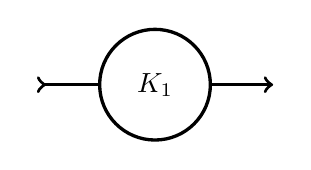
\begin{tikzpicture}[every path/.style={very thick}]
          \node[draw,circle,minimum size=40pt] (A) at (0,0) {$K_1$};
          \node (L) at (-1.5,0) {};
          \node (R) at (1.5,0) {};

          \draw[>-] (L.center) -- (A);
          \draw[->] (A) -- (R.center);
        \end{tikzpicture}
      \end{aligned} \times
      \begin{aligned}
        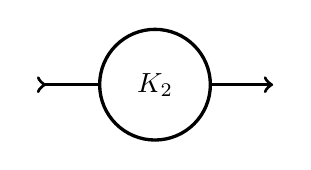
\begin{tikzpicture}[every path/.style={very thick}]
          \node[draw,circle,minimum size=40pt] (A) at (0,0) {$K_2$};
          \node (L) at (-1.5,0) {};
          \node (R) at (1.5,0) {};

          \draw[>-] (L.center) -- (A);
          \draw[->] (A) -- (R.center);
        \end{tikzpicture}
      \end{aligned} =
      \begin{aligned}
        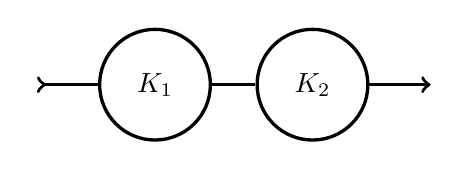
\begin{tikzpicture}[every path/.style={very thick}]
          \node[draw,circle,minimum size=40pt] (A) at (0,0) {$K_1$};
          \node[draw,circle,minimum size=40pt] (B) at (2,0) {$K_2$};
          \node (L) at (-1.5,0) {};
          \node (R) at (3.5,0) {};

          \draw[>-] (L.center) -- (A);
          \draw (A) -- (B);
          \draw[->] (B) -- (R.center);
        \end{tikzpicture}
      \end{aligned}
      \]
      \caption{The two-leg sum operation $\times$. If both $A$ and $B$ are two-leg-prime, then $A \times B$ has
        exactly one separating edge.}
      \label{fig:legsum_example}
    \end{figure}
    Hence, we will take $\ArbSubClass$ to be the class of knot shadows
    which remain at least 2-connected after removing the root edge.

    Certainly $A \times B \in \KnotShad$ as we obtain a new 2-leg shadow. As $\times$ introduces no
    crossings, we have $k = 0$ and $|A \times B| = |A| + |B|$. Finally, a 2-leg shadow $K$ either lies in
    $\ArbSubClass$ or has $\ell-1$ disconnecting edges. Cutting these edges produces the disjoint
    union of $\ell$ well-ordered 2-leg shadows (well ordered from their position in the long curve $K$)
    which is the unique ordered $+$-decomposition of $K$ into elements of $\ArbSubClass$.

    Let $\varphi$ be the map which twists the root edge, making the loop the new root (using the
    appropriate induced orientation). Then $\varphi: \KnotShad_* \hookrightarrow \ArbSubClass_{*+1}$,
    since deleting the root and smoothing the pointed edge produces a knot shadow, which must be at
    least 2-connected.
    \begin{figure}[h!]  \centering
      \[
      \begin{aligned}
        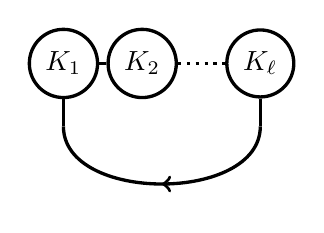
\begin{tikzpicture}[every path/.style={very thick},decoration={markings, mark=at position 0.5 with
        {\arrow{>}}}]
          \node[draw,circle,minimum size=15pt] (A) at (0,0) {$K_1$};
          \node[draw,circle,minimum size=15pt] (B) at (1,0) {$K_2$};
          \node[draw,circle,minimum size=15pt] (C) at (2.5,0) {$K_\ell$};
          \node (L) at (0,-.8) {};
          \node (R) at (2.5,-.8) {};

          \draw (L.center) -- (A);
          \draw (A) -- (B);
          \draw[dotted] (B) -- (C);
          \draw (C) -- (R.center);
          \draw (R.center) edge[out=-90,in=-90,postaction={decorate}] (L.center);
        \end{tikzpicture}
      \end{aligned} \xmapsto{\varphi}
      \begin{aligned}
        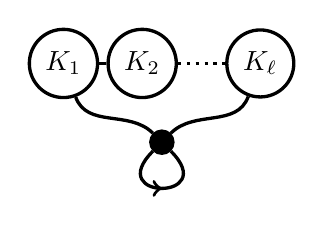
\begin{tikzpicture}[every path/.style={very thick},decoration={markings, mark=at position 0.5 with
        {\arrow{>}}}]
          \node[draw,circle,minimum size=15pt] (A) at (0,0) {$K_1$};
          \node[draw,circle,minimum size=15pt] (B) at (1,0) {$K_2$};
          \node[draw,circle,minimum size=15pt] (C) at (2.5,0) {$K_\ell$};
          \node[draw,circle,fill=black,minimum size=8pt,inner sep=0pt] (X) at (1.25,-1) {};

          \draw (X) edge[in=-70,out=90+45] (A);
          \draw (A) -- (B);
          \draw[dotted] (B) -- (C);
          \draw (C) edge[out=-110,in=90-45] (X);
          \draw (X) edge[out=-135,in=-45,postaction={decorate},looseness=10] (X);
        \end{tikzpicture}
      \end{aligned} \xmapsto{\varphi}
      \begin{aligned}
        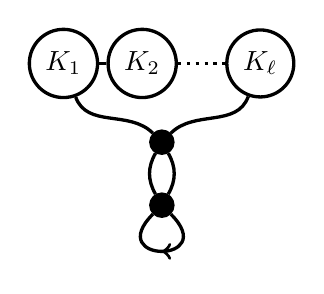
\begin{tikzpicture}[every path/.style={very thick},decoration={markings, mark=at position 0.5 with
            {\arrow{>}}}]
          \node[draw,circle,minimum size=15pt] (A) at (0,0) {$K_1$};
          \node[draw,circle,minimum size=15pt] (B) at (1,0) {$K_2$};
          \node[draw,circle,minimum size=15pt] (C) at (2.5,0) {$K_\ell$};
          \node[draw,circle,fill=black,minimum size=8pt,inner sep=0pt] (X) at (1.25,-1) {};
          \node[draw,circle,fill=black,minimum size=8pt,inner sep=0pt] (Y) at (1.25,-1.8) {};

          \draw (X) edge[in=-70,out=90+45] (A);
          \draw (A) -- (B);
          \draw[dotted] (B) -- (C);
          \draw (C) edge[out=-110,in=90-45] (X);
          \draw (X) edge[bend right] (Y);
          \draw (X) edge[bend left] (Y);
          \draw (Y) edge[out=-45,in=-135,postaction={decorate},looseness=10] (Y);
        \end{tikzpicture}
      \end{aligned}
      \]
      \caption{The map $\varphi$ adds a vertex and ensures that the new map is 2-leg-prime.}
      \label{fig:phi_example}
    \end{figure}
    Then we take $\psi_0 = \varphi$ and $\psi_1 = \varphi^2$. This setup satisfies the hypotheses
    and hence proves the theorem.
\end{proof}

\begin{corollary}
  There exists $N \ge 0$ and a constant $d < 1$ so that for $n \ge N$,
  \[\Prb(\text{a knot diagram $K$ is an unknot}) < d^n.\]

  For any prime 2-tangle $P$, there exists $N \ge 0$ and constants $d < 1$, $c > 0$ so that for
  $n \ge N$,
  \[\Prb(\text{a knot diagram $K$ contains $\le cn$ copies of $P$ as connect summands}) < d^n.\]
\end{corollary}

\begin{proof}
  The first statement will follow immediately from the second.

  %%% this won't work, probably should prove everything for rooted diagrams
  Let $k_n$ count the number of knot shadows with $n$ vertices and
  $h_n$ count the number of knot shadows in $n$ vertices which contain
  $\le c'n$ copies of $\Shad{P}$, where $c' > 0, d < 1, N$ are chosen
  by the corollary so that for all $n \ge N$, $h_n/k_n < d^n$. Then
  the number of rooted knot diagrams in $n$ crossings is $2^{n}$,
  and the number of rooted knot diagrams that contain $\le c'n$
  copies of $P$ is $2^{n-c'n}$ (there are two choices of orientation
  and $2^n$ choices of crossing sign, but $c'n$ of those are fixed if
  $P$)
\end{proof}

\subsubsection{Smooth growth for prime knot and link diagrams}
\label{sec:smoothprime}

If, however, we are considering a class $\PrimeShad$ of prime or reduced rooted diagrams, the method
of proof for smoothness does not immediately carry over; it is possible that $\varphi$ introduces
numerous isthmi, in which case our diagrams created in the final step would not even be reduced. If
$\PrimeShad$ is the case of prime rooted link shadows exact counts are known from their bijection
with simple quadrangulations~\cite{AlbenqueSQT};
\[ s_n = \frac{4(3n)!}{n!(2n + 2)!}.\]
In other cases again smoothness is more complicated to prove, although we can use a similar argument
to that in the case of all knot shadows.

\begin{proof}
  Step i is again immediate, so we begin with step ii. Let $\psi, \psi'$ respectively be maps which
  take the root vertex to the two 4-tangle shadows:

  Observe that neither $\psi$ nor $\psi'$ remove primeness or reducedness. Their images provide an
  injection into the spaces with 2 and 3 additional crossings, respectively. So take $m$
  appropriately.

  Define the operation $+$ now by the detour-glom. Notice that primeness is preserved and the
  process is splittable; given the root edge we can identify the bendy edges and rebuild the old two
  shadows. Notice that $|A + B| = |A| + |B| + 4$. Now let $C_3 \ge 1$ and $C_2 = C_3(r +
  \delta)^{-4}$. Then if there exist nonnegative integers $a, b$ such that $n = am + b(m+1) + (a+b)4
  = a(m + 4) + b(m+5)$, i.e.\ if $n \ge (m+4)(m+5)$, then
  \[ p_n > p_{m+4}^ap_{m+5}^b > C_2^{a+b}(r+\delta)^{-(am+b(m+1))} > C_3^{a+b}(r+\delta)^{-(a(m+4) + b(m+5))}
  > C_3(r+\delta)^{-n}.\]
\end{proof}

\subsection{Asymmetry of diagrams and consequences}
\label{sec:asymmetry}


The following theorem of Richmond and Wormald \cite{Richmond19951} provides a sufficient set of
criteria for almost all elements of $\FlatKnotDia$ to have trivial automorphism group.
\begin{theorem}[Richmond-Wormald 1996]
  Let $\mathscr C$ be a class of rooted maps on a surface. Suppose that there is an outer-cyclic
  rooted planar map $M_1$ such that in all maps in $\mathscr C$, all copies of $M_1$ are pairwise
  disjoint, and such that
  \begin{enumerate}
  \item $M_1$ has no reflective symmetry in the plane preserving the unbounded face,
  \item there exist constants $c > 0$ and $d < 1$ such that the proportion of $n$-vertex maps in
    $\mathscr C$ that do not contain at least $cn$ pairwise disjoint copies of $M_1$ is at most
    $d^n$ for $n$ sufficiently large ($M$ is ``ubiquitous''), and
  \item for any map $M$ in $\mathscr C$ containing a copy of $M_1$, all maps obtainable by removing
    $M_1$ and gluing it back in to the same face are in $\mathscr C$ ($M$ is ``free'').
  \end{enumerate}
  Then the proportion of $n$-vertex maps in $\mathscr C$ with nontrivial automorphisms is
  exponentially small.
\end{theorem}

We will prove this for $\FlatKnotDia$ by proving it for its dual $\FlatKnotDia^*$, a class of
quadrangulations of the sphere. Specifically, we will take $M_1$ to be the dual of the underlying
planar map of the following 2-tangle:
\begin{figure}[h!]
  \centering
  \begin{tikzpicture}[every path/.style={string, very thick}, every node/.style={transform shape,
      knot crossing, inner sep=1.5pt}]
    \node (tl) at (-.7,0) {};
    \node (tr) at (.7,0) {};
    \node (tc) at (0,1) {};
    \node (el) at (-1.7,0) {};
    \node (er) at (1.7,0) {};
    \node (r1) at (.9,1.2) {};
    \draw[>-] (el.center) .. controls (el.4 east) and (tl.4 south west) .. (tl);
    \draw (tl) .. controls (tl.4 north east) and (tc.4 south west) ..  (tc.center);
    \draw (tc.center) .. controls (tc.4 north east) and (r1.4 south
    west) .. (r1);
    \draw (r1) .. controls (r1.16 north east) and (r1.16 north west)
    .. (r1.center);
    \draw (r1.center) ..controls (r1.4 south east) and (tr.4 north
    east) .. (tr);
    \draw (tr) .. controls (tr.4 south west) and (tl.4 south east)
    .. (tl.center);
    \draw (tl.center) .. controls (tl.8 north west) and (tc.8 north
    west) .. (tc);
    \draw (tc) .. controls (tc.4 south east) and (tr.4 north west)
    .. (tr.center);
    \draw[->] (tr.center) .. controls (tr.4 south east) and (er.4 west)
    .. (er.center);
  \end{tikzpicture}
  \caption{The dual 2-tangle $M_1$, and its representation as a 2-tangle.}
  \label{fig:treflegs2}
\end{figure}
Clearly $M_1$ has no reflective symmetry by inspection, and certainly any of the ways of replacing
$M_1$ keep the object in the class of quadrangulations dual to knot maps. Finally, the ubiquity
condition is exactly the pattern theorem for 2-tangles proved in the prior section!

Application of the above theorems provides us with the following corollary which enables us to
transfer any asymptotic results on rooted diagrams to unrooted diagrams.

\begin{corollary}
  Let $L$ be a uniform random variable taking values in the space $\KnotDia_n$ or $\LinkDia_n$. Then
  there exist constants $C, \alpha > 0$ so that $\Prb(\Aut L \ne 1) < Ce^{-\alpha n}$. Hence, rooted
  diagrams behave like unrooted diagrams.
\end{corollary}

Indeed, link diagrams with $n$ vertices are dual to quadrangulations with $n+2$ faces; there are
$n+2$ ways of choosing the ``exterior'' root face and then $4$ ways of rooting the edges around this
chosen face. Hence if $\tilde \ell_n$, $\tilde k_n$ are the counts of unrooted link or knot diagrams
we have that in the limit,
\[ \tilde\ell_n \underset{n\to\infty}{\sim} \frac{\ell_n}{4(n+2)} \text{ and } \tilde k_n
\underset{n\to\infty}{\sim} \frac{k_n}{4(n+2)}.\]

\begin{corollary}
  A random knot or link diagram has the pattern theorem. Namely, a random knot diagram is almost
  surely composite and almost surely knotted, and a random link diagram is almost surely not a knot
  diagram.
\end{corollary}

\section{Numerical results on knotting}
\label{sec:randres}

One may be concerned that the ``asymptotic'' behavior proved in the prior section only applies to
knot diagrams with an absurd number of crossings (in the sense that no physical knot should be
expected to be so complicated). However, exact and numerical results show that this behavior is
attained very quickly. For example, almost all 10-crossing knot diagrams have no nontrivial
automorphisms!

\bibliography{sources.bib}

\end{document}

%%% Local Variables:
%%% mode: latex
%%% TeX-master: t
%%% End:
